\section{Results and Discussion}
\label{results}

We present now the results obtained by each study performed. 

\subsection{Case Study}

Table~\ref{tab:caseStudyResults} presents the results of applying \contractjdoc{} to each system.
Column \#Clauses displays the number of clauses manually added in each system.
Column \#Errors presents the number of errors detected by the systems test suite after compiling the source code enhanced with contracts in
\contractjdoc{} approach. Column Time reveals the time (in seconds) needed for compiling the whole
project with its dependencies after applying \contractjdoc{} contracts. Columns \#Com.Case to \#Repet.
show the contract clauses added in each system grouped by type (following the
definitions from ~\cite{typeContracts}).

\begin{table*}[h]
\caption{Case study Results.}
\label{tab:caseStudyResults}
\centering
\begin{tabular}{l l l l l l l l}
\hline
 \bfseries System &
 \bfseries \#Clauses & 
 \bfseries \#Errors & 
 \bfseries Time (s) &
 \bfseries \#Tests &
 \bfseries \#Com.Case &
 \bfseries \#AppSpec. &
 \bfseries \#Repet. \\ \hline
ABC-Music-Player & 115 & 2 & 14 & 30 & 42 & 11 & 62 \\
Dishevelled & 2,655 & 381 & 434 & 2,643 & 1,536 & 151 & 968 \\
Jenerics & 190 & 7 & 20 & 44 & 156 & 0 & 34 \\
OOP Aufgabe3 & 54 & 1 & 4 & 11 & 16 & 30 & 8 \\
SimpleShop & 50 & 0 & 5 & 0 & 30 & 11 & 9 \\
Webprot\'{e}g\'{e} & 930 & 0 & 713 & 0 & 717 & 79 & 133 \\ \hline

 \bfseries Total & 
 \bfseries \totalClauses{} & 
 \bfseries 391 &
 \bfseries 1,185 &
 \bfseries 2,728 &
 \bfseries 2,497 &
 \bfseries 282 &
 \bfseries 1,214
\\
\bottomrule
\end{tabular}
\end{table*}

% Jenerics: 8 - 6 failures, 1 error.

% results for contract types
Concerning the kind of contracts, the only unit in which we wrote more
application-specific contracts was \texttt{OOP Aufgabe3} system (55\% of the
written contracts are application-specific). On the other hand, in \texttt{ABC-Music-Player}, more than 90\% of the contracts remains between common-case and
repetitive code: verifications that strings are not blank, collections are not
empty, or that a method returns a field.
For \texttt{Dishevelled}, the majority of the written contracts is classified as common-case
(57.51\%), other 36.92\% are repetitive with code and only 5.57\% are application-specific.
In addition, all contracts written for \texttt{Jenerics} are related to
verification of nullity from parameters or the return value, thus all contracts
remains between common-case and repetitive code. In \texttt{SimpleShop}, the
written contracts are distributed in the following manner: common-case 60\%, repetitive code 19\%, and application-specific 21\%; again the number of common-case and repetitive code outperforms application-specific contracts. Finally,
in \texttt{WebProt\'{e}g\'{e}}, the distribution is: common-case 77.51\%, repetitive code 14.38\%, and application-specific 8.11\%.  

% conformance errors
When applying \contractjdoc{} to \texttt{ABC-Music-Player}, we found inconsistencies between Javadoc
comments and the source code. The problems occurred in the class \texttt{Utilities} (package
\texttt{sound}) because there are comments concerning a parameter declaring that the value of
this parameter must not be greater than or equal to zero; however in the body of the methods there
is an if-clause that throws exceptions when the value received by the parameter is negative.

\subsubsection{Case Study}
\label{sec:caseStudyDiscussion}

% applying contractjdoc
For all systems (see Table~\ref{tab:Units}), we
wrote more pre- and postconditions than invariants. This result has two
explanations: first, as expected the amount of Javadoc comments over the
classes' fields in the evaluated systems is low in comparison with the amount
of Javadoc comments over method's parameters and return.

%  -- the only
% exception occurred in \texttt{SimpleShop} system because the developers have used resources from Java
% constraints for declaring some fields as not null, enabling us to establish
% invariants for them; second, even when there are no comments in a method, we are
% able to write pre- and postconditions based on analysis of method's body.

Concerning pre- and postconditions, for \texttt{ABC-Music-Player} and
\texttt{WebProt\'{e}g\'{e}} projects, we wrote almost twice as many postconditions
as preconditions.
In \texttt{ABC-Music-Player} this is related to the number of accessor methods
available and for \texttt{WebProt\'{e}g\'{e}}, the difference is related to
the available comments.
%  and to the contracts we are able to infer from method's
% body.
%
% In addition, based on the comment and the body of a method, establishing a
% postcondition appears to be simpler than a precondition, as we do not know
% the methods' clients beforehand.


We were able to detect potential inconsistencies in \texttt{ABC-Mu\-sic-Player};
the exception will be always thrown, differently from what is expected from the
commentary.
We also found a problem into
\texttt{WebProt\'{e}g\'{e}} project, in the class \texttt{OWLLiteralParser} there was one exception
in the Javadoc tag \texttt{@throws} that was not declared in the throws of the method's signature.

% conformance errors
In addition, sometimes the tests available along with the systems do
not respect the definitions from the Javadoc comments. For instance, when the
comments in natural language from \texttt{ABC-Music-Player} system are turned into
\contractjdoc{} contracts, some tests from
\texttt{MainTest}, \texttt{ParserTest}, and \texttt{SequencePlayerTest} violate
the methods' preconditions from class \texttt{Utilities}, they try to
call \texttt{Utilities}' methods by passing the value zero as the second
parameter, even though the comment declares the second parameter must be greater than zero.
This scenario also occurred in \texttt{Dishevelled} unit, the comments turned
in \contractjdoc{} contracts also enable us to detect some tests
that do not respect the restrictions available in the Javadoc comments.

As a proof of concept, \contractjdoc{} and its compiler (\contractjdocCompiler{}) enabled us to write runtime
checkable code for third-party systems based on the comments in natural
language.
As expected, the quality and variety of the contracts depended strongly on the available comments, however, we were able to
detect and correct inconsistencies and missing expressions between source code and comments.




\subsection{Empirical Study}
\label{sec:expResults}

27 Java developers participated in our experiment. From those, we 
randomly discarded three in order to maintain a balanced
number of participants in each trial. Thus, we maintained 24 developers, from those, 
10 are working in industry (41.6\%) and 14 are students (58.4\%).


% difficulty
Concerning the task performed by the developers, we present in
Figure \ref{fig:tasksEmpirical}
answers on difficulty grouped by the task performed.
The implementation of the documented interface (Supplier task) seemed to be easier
than the task of creating a Client class, however, this difference is not
statistically significant as presented by a Wilcoxon rank sum test~\cite{statistical}
(p-value = 0.07, confidence level of 95\%).
%

\begin{figure*}
\centering
\begin{subfigure}{.3\textwidth}
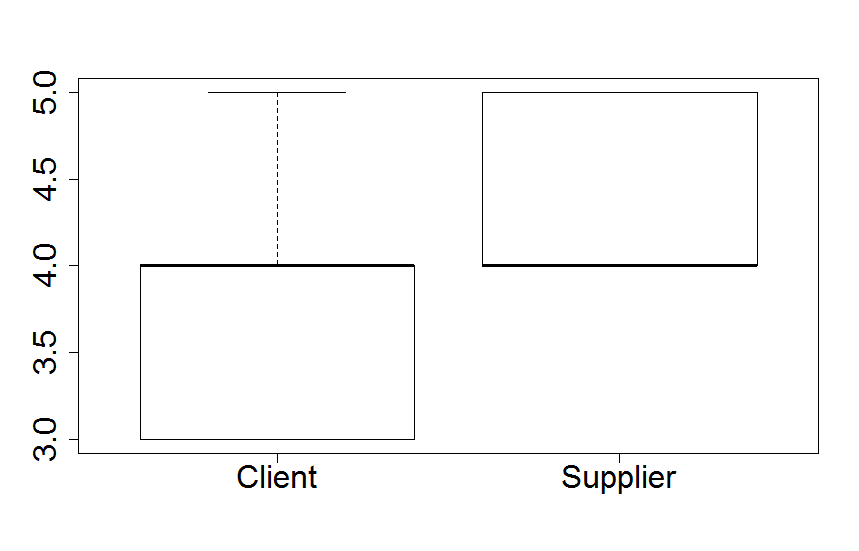
\includegraphics[width=1\linewidth]{figs/boxplotTasksEmpiricalStudy}
\caption{}
\label{fig:tasksEmpirical}
\end{subfigure}
\begin{subfigure}{.3\textwidth}
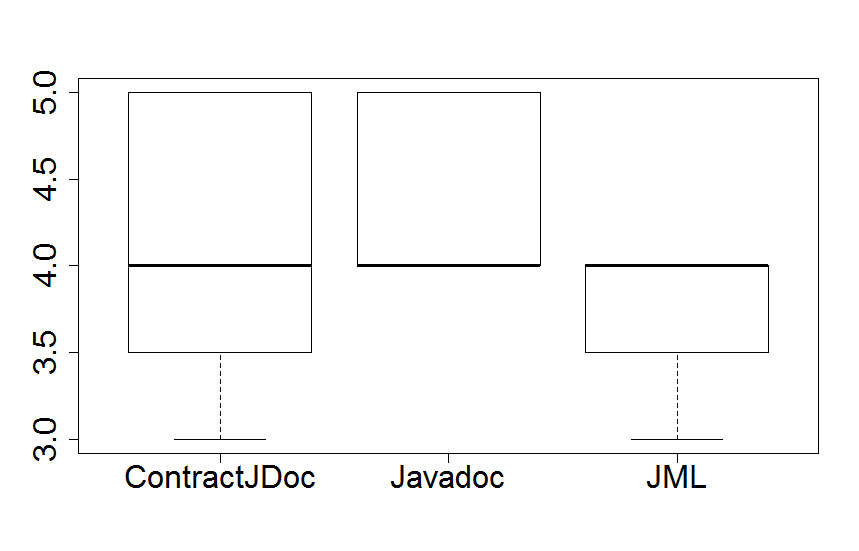
\includegraphics[width=1\linewidth]{figs/boxplotApproachesEmpiricalStudy}
\caption{}
\label{fig:approachesEmpirical}
\end{subfigure}
\begin{subfigure}{.3\textwidth}
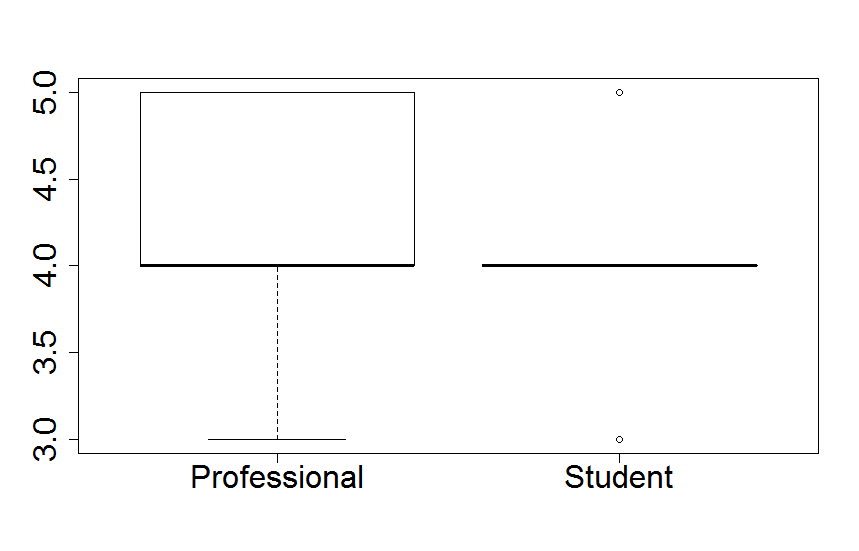
\includegraphics[width=1\linewidth]{figs/boxplotExperienceEmpiricalStudy}
\caption{}
\label{fig:experienceEmpirical}
\end{subfigure}
\caption{Results of our empirical study with Java developers, on an implementation task based on a
documented-interface, aiming to evaluate the readability and understandability of three approaches
for documenting Java code.}
\label{fig:empiricalResults}
\end{figure*}


% \begin{figure}
% \centering
% 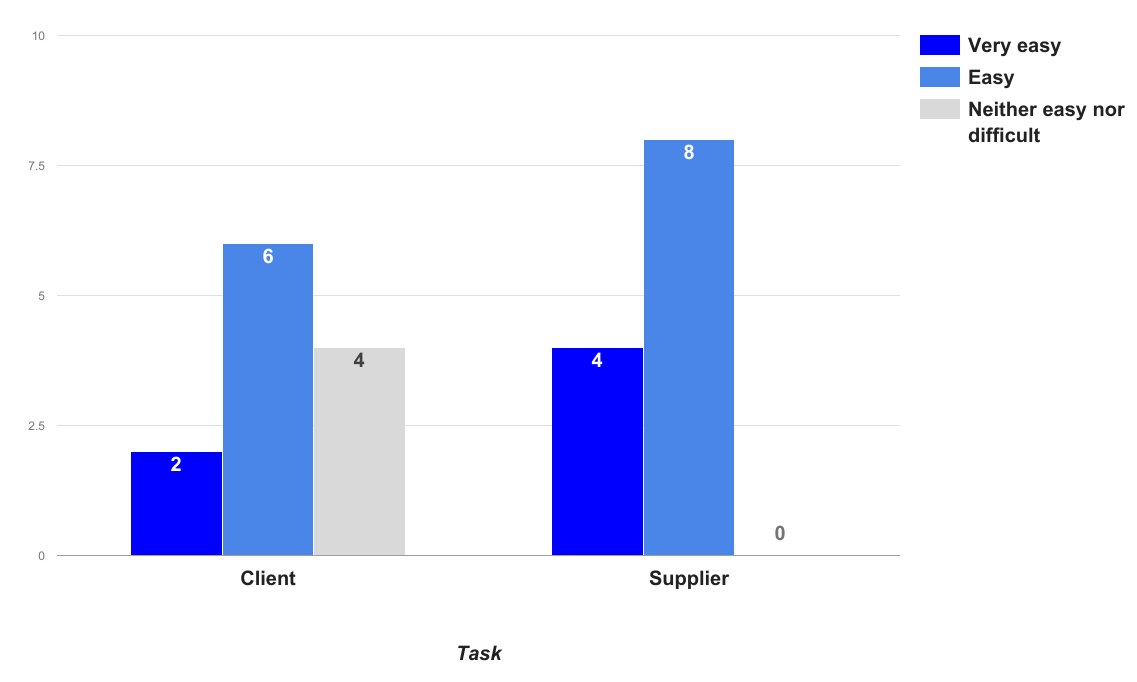
\includegraphics[width=1.0\textwidth]{figs/TaskComplexity}
% \caption{Answers grouped by task complexity.}
% \label{fig:taskComplexity}
% \end{figure}

% documenting approach
When grouped by documenting approach (see Figure \ref{fig:approachesEmpirical}),
the Kruskal-Wallis rank sum test showed no difference between the approaches
(p-value = 0.15).

% , the results present Javadoc as the easiest approach to be understood (see Figures \ref{fig:empiricalResults}(c),
% \ref{fig:empiricalResults}(d), and \ref{fig:empiricalResults}(e)). This is
% expected since Javadoc is a well established approach for documenting Java code. In addition, \contractjdoc{} was perceived as easier than JML: there are three answers \textit{Very easy} for \contractjdoc{} whereas
% there is no answer \textit{Very easy} for JML.

% experience
When grouped by experience (Figure \ref{fig:experienceEmpirical}), the Wilcoxon
rank sum test (p-value = 0.45) also does not show differences statistically
significant between professionals and students. 

% source code correct
Javadoc and \contractjdoc{} were the only documenting approaches in
which all participants were able to produce a code satisfying the oracle
(respecting the restrictions available in the comments). On the other hand,
there was one case developed by following the JML documenting approach in which
the contract is not satisfied by the implementation.

\subsubsection{Empirical Study}
\label{sec:expDiscussion}

We proceed with the discussion over the research questions.

% task
\textbf{Q2.} We ask each developer to perform one task:
either implement a given interface or implement a client code for using the
methods provided by an interface -- such the use of an API (Client). 
Although developers have assigned more \emph{Very Easy} and \textit{Easy} for
the supplier task than to the client (see Figure~\ref{fig:empiricalResults}(a)),
the statistical test did not provide evidences for a significant difference
between the difficulty perceived by developers when performing the required
task.


% approach
\textbf{Q3.}  Although not supported by statistical tests since Kruskal-Wallis
rank sum test showed no difference between the approaches (p-value = 0.15), Javadoc and
\contractjdoc{} were perceived as being easier than JML (see Figure~\ref{fig:approachesEmpirical}).
This result indicates \contractjdoc{} as an approach in an intermediate level
between Javadoc and JML, with both providing runtime conformance checking. Therefore, the
proposed approach is promising: \contractjdoc{} is easy to understand
(create a code based on the comments) -- 75\% of the developers answers for
difficulty remains between \textit{Easy} and \textit{Very easy} -- and enables
the runtime checking of the comments by means of \contractjdocCompiler{}
compiler.

%code correctness
\textbf{Q4.} Concerning the code correctness, all Participants using
interfaces documented with Javadoc and \contractjdoc{} produced code
in accordance with the contracts available in the interfaces. Only one
developer using an interface with JML contracts was not able to
satisfy all the contracts: in one method the source code produced is not in
conformance with the contracts. 

% kind of task
Even though the developers have been perceived the supplier task as less
difficult than the client task, they produced code respecting the restrictions
available on the comments more times to the client task. All developers were
able to write a client code in accordance with the restrictions. Maybe the
difficulty reported by the developers is related with the attention required for
using methods provided by an interface: one needs to read the documentation
available in order to know how to use the methods; whereas implementing the
interface is more simple; mainly for the interfaces used in this experiment:
they are traditional and well-known data structures.
The results of this experiment suggest that when writing a client code,
developers tend to pay more attention to the documentation available than when
they are writing a supplier code (implementing a given interface).





\subsection{Comprehensibility Survey}
\label{sec:surveyResults}

142 Java developers answered the survey.
From those, 
51 are professionals (36\%) and 91 are students
(64\%).

%results - in general
With respect to the survey answers, 50.7\% (72) of the Subjects chose Javadoc as
the simplest approach to understand when using it in a general context. In addition,
for 38\% (54) of the subjects Javadoc is also the most understandable approach
with regard to the provided interface.

\begin{figure*}
\centering
\begin{subfigure}{.48\textwidth}
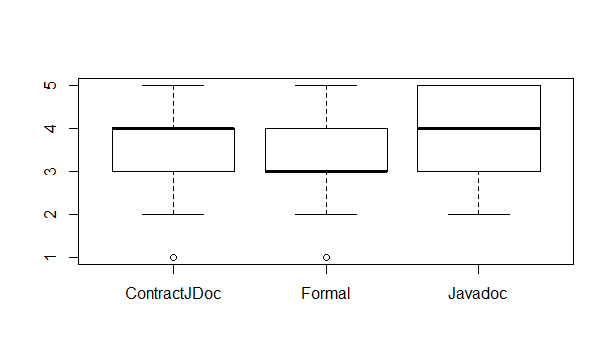
\includegraphics[width=1\linewidth]{figs/boxplotApproachesSurveyStudy}
\caption{All approaches}
\label{fig:allApproaches}
\end{subfigure}
\begin{subfigure}{.48\textwidth}
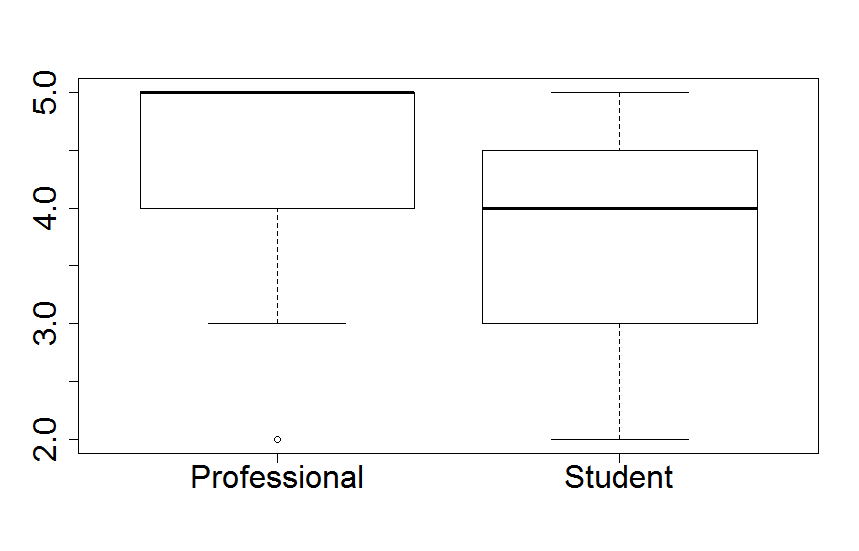
\includegraphics[width=1\linewidth]{figs/boxPlotJavadocXExperience}
\caption{Javadoc}
\label{fig:javadocExp}
\end{subfigure}
\\[1ex]
\begin{subfigure}{.48\textwidth}
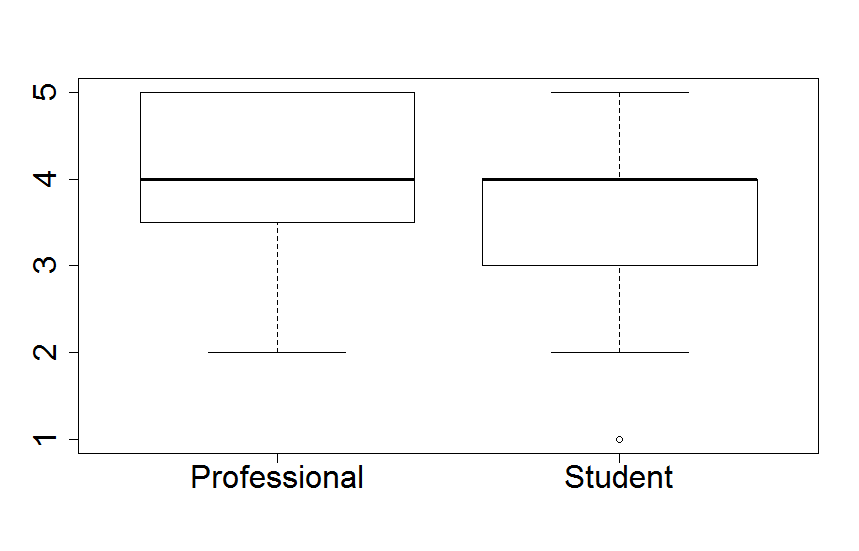
\includegraphics[width=1\linewidth]{figs/boxplotContractJDocXExperience.png}
\caption{\contractjdoc{}}
\label{fig:contractjdocExp}
\end{subfigure}
\begin{subfigure}{.48\textwidth}
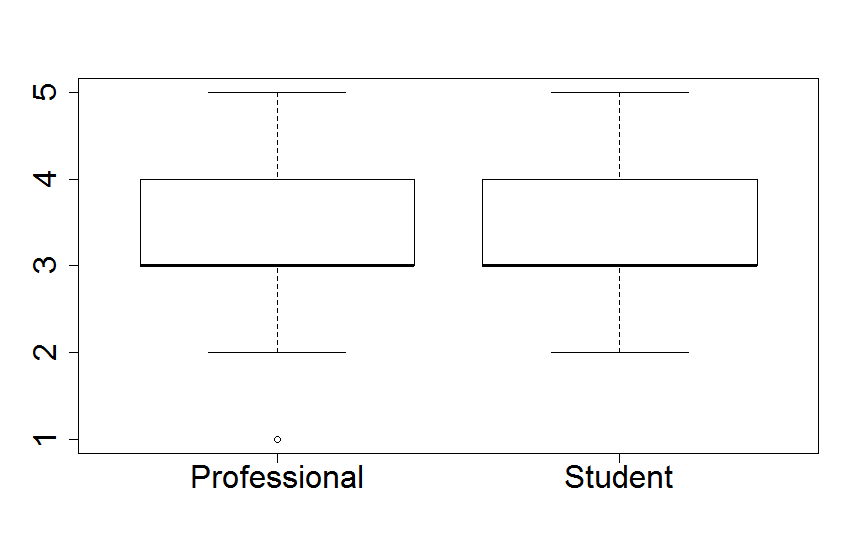
\includegraphics[width=1\linewidth]{figs/boxplotJMLXExperience.png}
\caption{JML}
\label{fig:jmlExp}
\end{subfigure}
\caption{Subjects' answers to the individual evaluation of comprehensibility for
each documentation approach. And answers grouped by experience for each
approach.}
\label{fig:surveyResults}
\end{figure*}

% continues
The survey results provided us statistical difference when comparing the the
comprehensibility of the documentation approaches evaluated (see
Figure~\ref{fig:allApproaches}). By performing an Oneway ANOVA test~\cite{statistical} and
a corresponding post hoc analysis we were able to distinguish the three
approaches (p-value $<$ 0.05).
The Tukey HSD~\cite{statistical} and pairwise comparisons using t tests
with Bonferroni correction~\cite{statistical} produced the following p-values:
Javadoc-ContractJDoc = 0.012, JML-ContractJDoc = 0.000, and JML-Javadoc = 0.000.

When analyzing data grouped by experience (Figures~\ref{fig:javadocExp} to
~\ref{fig:jmlExp}) by means of Wilcoxon rank sum test with continuity correction
tests, only for JML we found no statistical difference between Professionals and
Students (p-value = 0.17). For both Javadoc and \contractjdoc{}, Professionals
had perceived the approaches as being easier for comprehensing than Students
(p-value = 0.012 and p-value = 0.004, respectively).

\subsubsection{Comprehensibility Survey}
\label{sec:surveyDiscussion}

According to the statistical tests performed, Javadoc is the most
understandable documentation approach, and \contractjdoc{} is intermediate between JML and
Javadoc, being closer to Javadoc.
This can also be seen in Figure~\ref{fig:allApproaches}.

An interesting result came from the analysis of the difficulty grouped by
experience (Figures~\ref{fig:javadocExp} to ~\ref{fig:jmlExp}): students and
professionals have perceived the same level of difficulty for JML, which is
promissing as contract-based languages are usually considered harder to be
understood by people with less experience (students, in our survey).

Overall, this survey corroborate with the results from our experiment: \contractjdoc{} is
intermediate between Javadoc and JML, being closer to Javadoc with respect to
comprehensibility.
Furthermore, the results highlight Javadoc as the easiest approach concerning the comprehensibility of
the behavior of a documented interface.
